When developing this measurement strategy, I found myself curious about the quality level of some cross sections of Wikipedia where there were once known content coverage gaps.  I decided to focus on coverage of women scientists in Wikipedia.  Regretfully, Wikipedia's category\footnote{See \url{https://www.mediawiki.org/wiki/Help:Categories}} structure is notoriously useless for drawing meaningful cross sections of content~\cite{kittur09what}.  Luckily, WikiProject organizers are keen on making sure that all aticles about within their topic space are tagged and tracked by their project templates\footnote{See \url{https://www.mediawiki.org/wiki/Help:Templates}}. So searching for the presence of WikiProject Women Scientist templates is an efficient means for gathering this cross section\footnote{See \url{https://quarry.wmflabs.org/query/14033} for the query and its result.}.  Note that this method can be used to derive cross sections for any other WikiProject topic space.

As described in the previous section, I generated aggregate metrics both for the entire Wikipedia (about 5 million articles) and just the articles covering women scientists (5,681).  I then compared the aggregated measures for \emph{mean weighted sum} and proportion of articles in each quality class to look for shifts in the quality gap (when the apparent quality of articles about women scientists is lower than the apparent quality of the rest of the encyclopedia) and surplus (the opposite).

\begin{figure*}[p]
\centering
\begin{subfigure}[t]{\columnwidth}
  \centering
  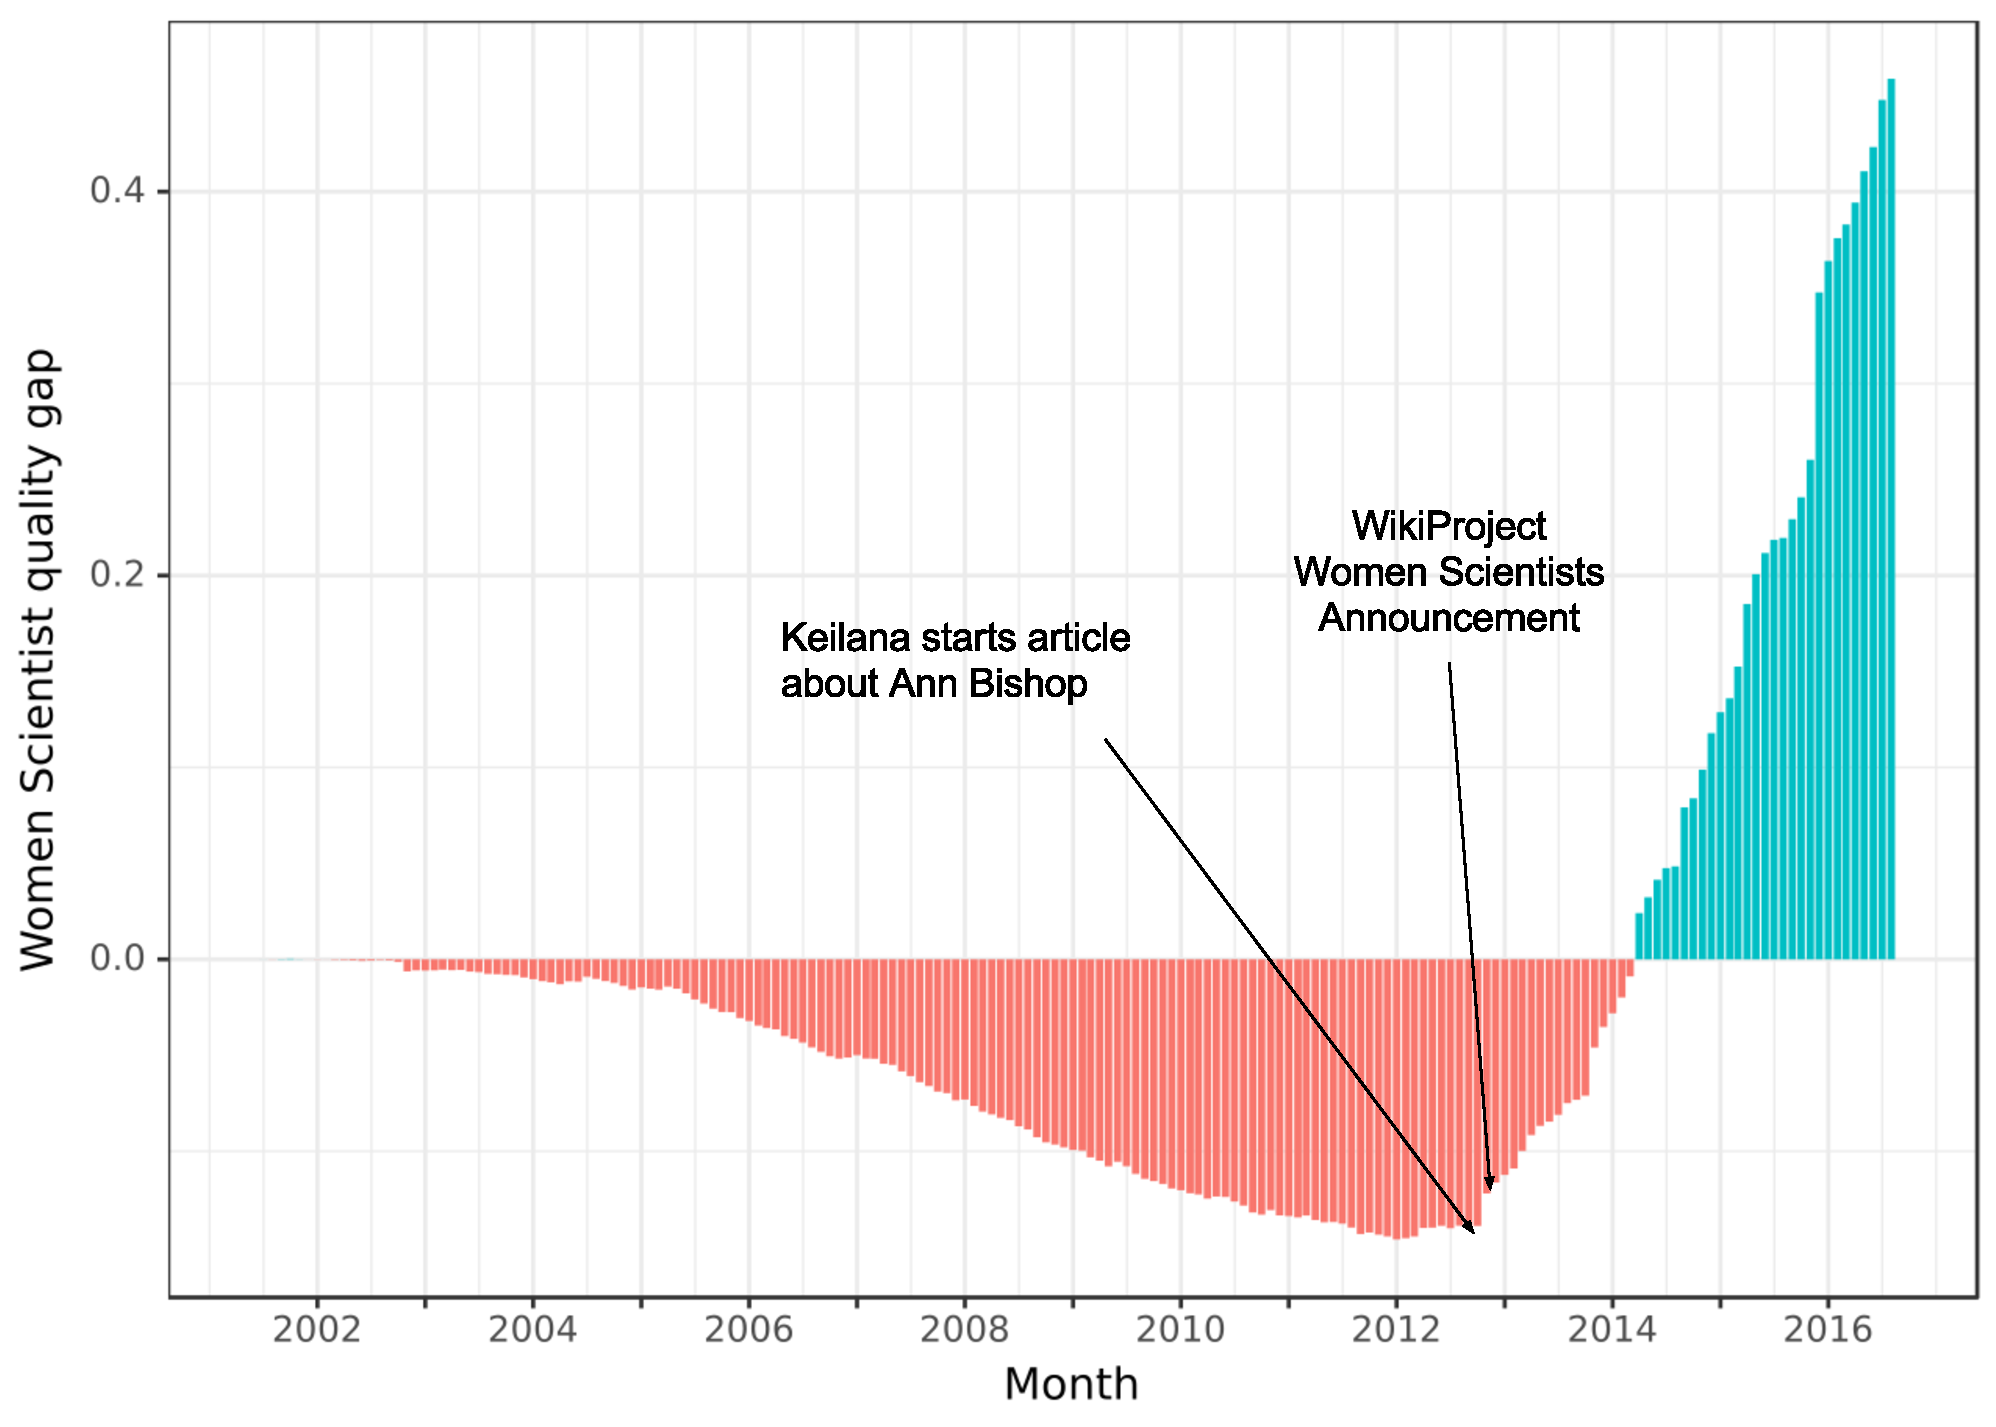
\includegraphics[width=.9\textwidth]{figures/mean_weighted_sum_ws_vs_all}
  \caption{The difference in \emph{mean weighted sum} quality predictions for all wiki and articles about Women Scientists is plotted over time. Note the transition from red to blue represents the switch from a gap to a surplus.  Important dates for User:Keilana's initiatives are annotated with arrows.}
  \label{fig:mean_weighted_sum_ws_vs_all}
\end{subfigure}\\
\begin{subfigure}[t]{\columnwidth}
  \centering
  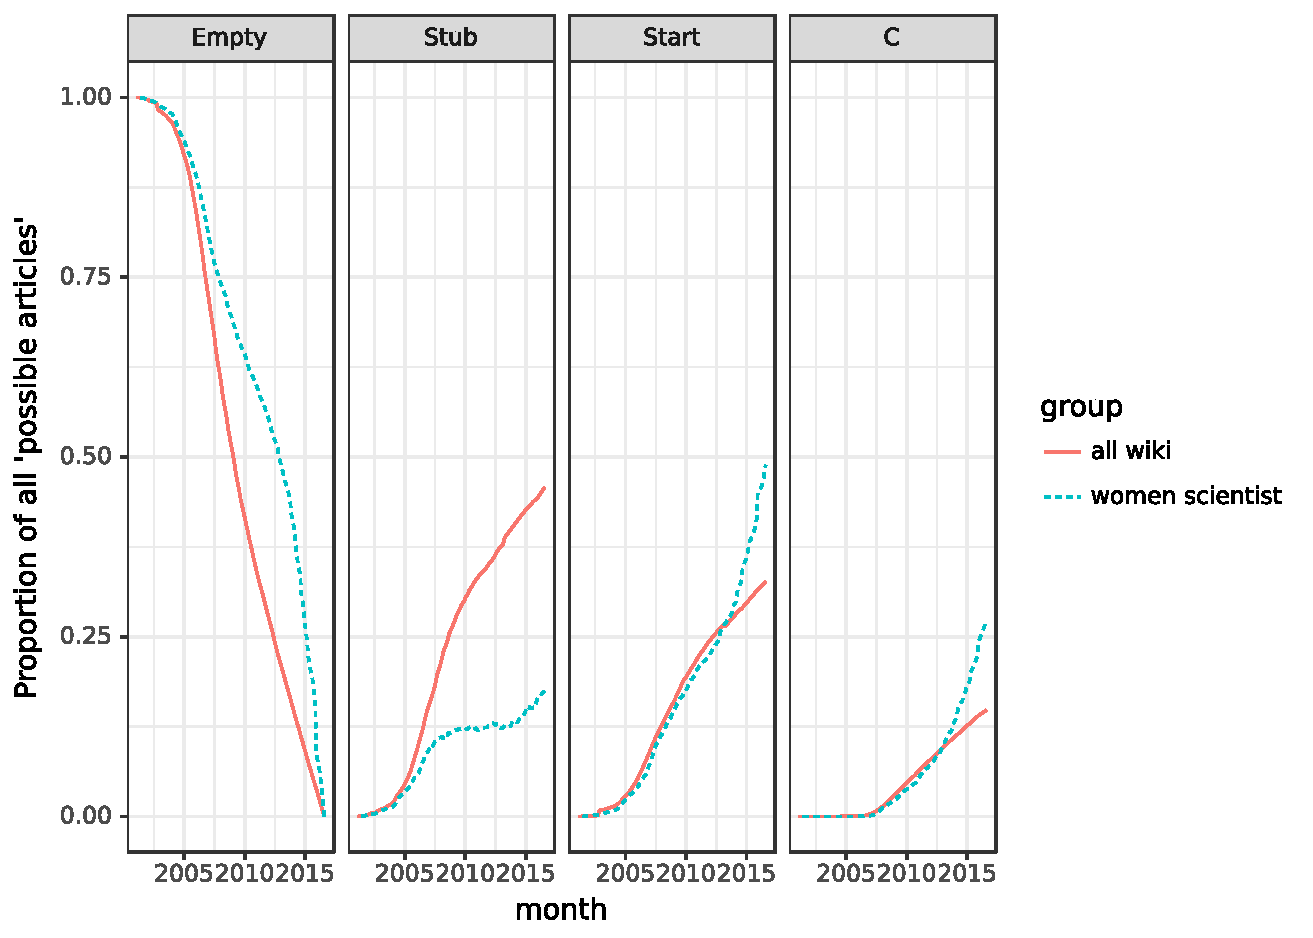
\includegraphics[width=.9\textwidth]{figures/proportion_empty2c_ws_vs_all}
  \caption{The proportion of articles falling into Empty, Stub, Start, and C-class predictions is plotted for articles tagged by WikiProject Women Scientists and all of Wikipedia.}
  \label{fig:proportion_empty2c_ws_vs_all}
\end{subfigure}~~
\begin{subfigure}[t]{\columnwidth}
  \centering
  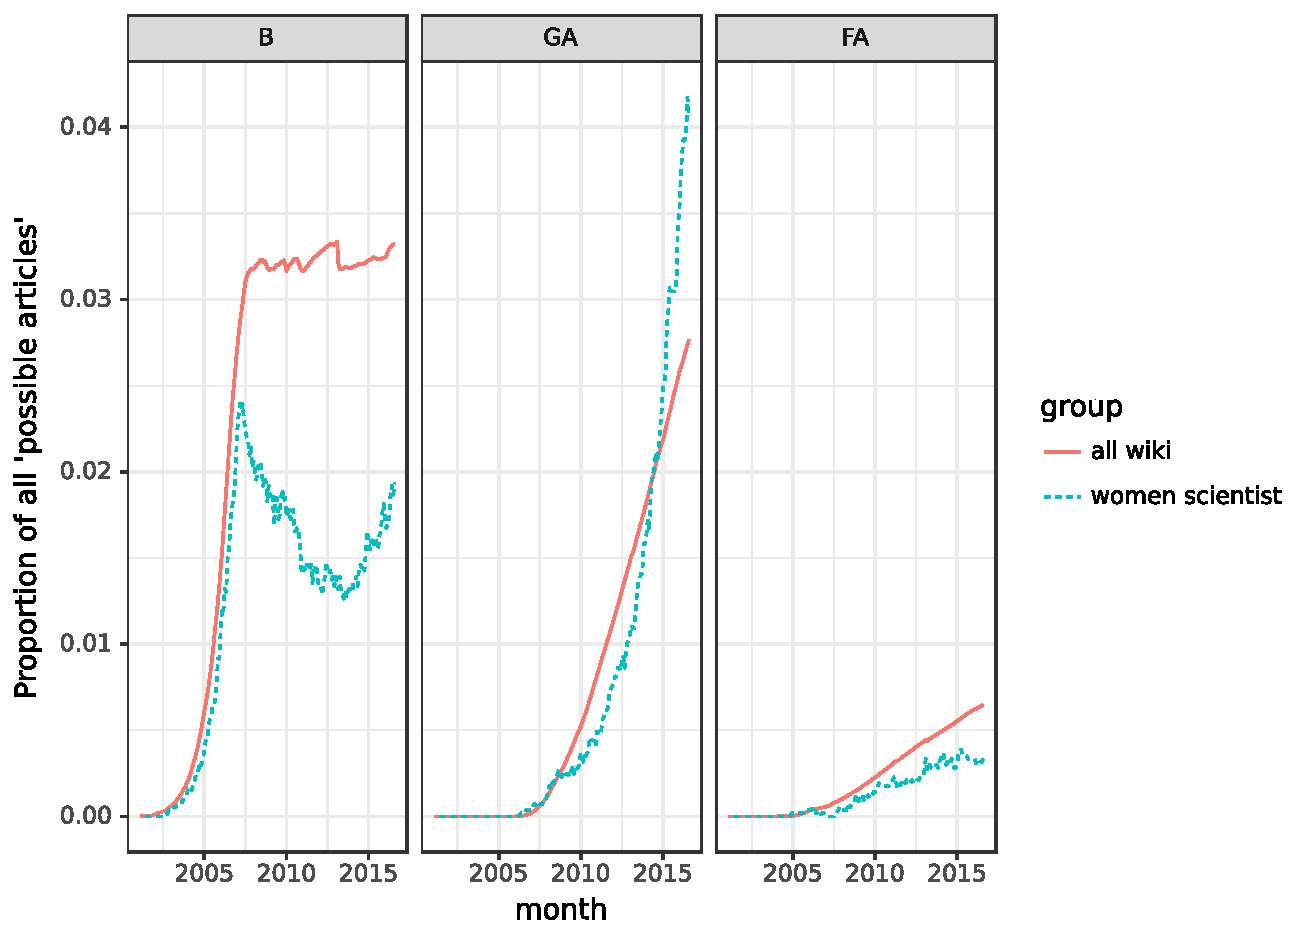
\includegraphics[width=.9\textwidth]{figures/proportion_b2fa_ws_vs_all}
  \caption{The proportion of articles falling into B, GA, and FA-class predictions is plotted for articles tagged by WikiProject Women Scientists and all of Wikipedia.}
  \label{fig:proportion_b2fa_ws_vs_all}
\end{subfigure}
\caption{The quality dynamics of biographies about women scientists vs. all of English Wikipedia.}
\label{fig:ws_vs_all}
\end{figure*}


Figure~\ref{fig:mean_weighted_sum_ws_vs_all} shows the difference between the ``mean weighted sum'' of article quality for all of Wikipedia and just the articles about women scientists.  From the start of Wikipedia, a gap quickly develops and reaches the maximum of about a 15\% a quality level around the middle of 2012.  But after that point, the gap starts to rapidly close and a massive surplus begins to grow to about half of a quality class above the rest of the encyclopedia.

This dynamic roughly plays out in the same way for the proportions of articles that fall into the higher predicted quality classes.  Figures~\ref{fig:proportion_empty2c_ws_vs_all} and \ref{fig:proportion_b2fa_ws_vs_all} clearly show that the proportion of Start, C, and GA-class articles shows a similar gap and surplus period.  Stub-class articles about women scientists seem to continue to fall behind the rest of the wiki, but there's still a noticeable increase in the proportion around the beginning of User:Keilana's initiatives (discussed in the \nameref{sec:discussion} section).  It seems that the growth dynamics of B-class articles is shaped very differently from the rest of the quality prediction classes.  Surprisingly, there seems to be no surplus in the proportion of articles that fall into FA-class.  It seems that this is the only quality class where no noticeable shift occurs -- the gap between women scientist biographies and the rest of Wikipedia only widens over time.
